\section*{Preface}

There are several popular meanings of the term \q{\gls{reverse engineering}}:
1) The reverse engineering of software: researching compiled programs;
2) The scanning of 3D structures and the subsequent digital manipulation required in order to duplicate them;
3) Recreating \ac{DBMS} structure.
This book is about the first meaning.

\subsection*{Topics discussed in-depth}

x86/x64, ARM/ARM64, MIPS, Java/JVM.

\subsection*{Topics touched upon}

\oracle (\myref{oracle}),
Itanium (\myref{itanium}),
copy-protection dongles (\myref{dongles}), 
LD\_PRELOAD (\myref{ld_preload}),
stack overflow,
\ac{ELF},
win32 PE file format (\myref{win32_pe}),
x86-64 (\myref{x86-64}),
critical sections (\myref{critical_sections}),
syscalls (\myref{syscalls}), 
\ac{TLS},
position-independent code (\ac{PIC}) (\myref{sec:PIC}), 
profile-guided optimization (\myref{PGO}),
C++ STL (\myref{cpp_STL}),
OpenMP (\myref{openmp}),
SEH (\myref{sec:SEH}).

\subsection*{Exercises and tasks}

\dots 
are all moved to the separate website: \url{http://challenges.re}.

\subsection*{About the author}
\begin{tabularx}{\textwidth}{ l X }

\raisebox{-\totalheight}{
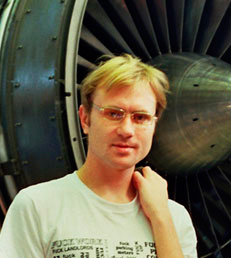
\includegraphics[scale=0.60]{Dennis_Yurichev.jpg}
}

&
Dennis Yurichev is an experienced reverse engineer and programmer.
He can be contacted by email: \textbf{\EMAIL{}}, or on Skype: \textbf{dennis.yurichev}.

% FIXME: no link. \tablefootnote doesn't work
\end{tabularx}

% subsections:
\subsection*{\RU{Отзывы о книге}\EN{Praise for} \IT{\TITLE}}

\begin{itemize}
\item ``It's very well done .. and for free .. amazing.''\footnote{\url{https://twitter.com/daniel_bilar/status/436578617221742593}} Daniel Bilar, Siege Technologies, LLC.

\item ``...excellent and free''\footnote{\url{https://twitter.com/petefinnigan/status/400551705797869568}} Pete Finnigan, \RU{гуру по безопасности }\oracle\EN{ security guru}.

\item ``... book is interesting, great job!'' Michael Sikorski, \RU{автор книги}\EN{author of} \IT{Practical Malware Analysis: The Hands-On Guide to Dissecting Malicious Software}.

\item ``... my compliments for the very nice tutorial!'' Herbert Bos, \RU{профессор университета}\EN{full professor at the} Vrije Universiteit Amsterdam.

\item ``... It is amazing and unbelievable.'' Luis Rocha, CISSP / ISSAP, Technical Manager, Network \& Information Security at Verizon Business.

\item ``Thanks for the great work and your book.'' Joris van de Vis, SAP Netweaver \& Security specialist.

\item ``... reasonable intro to some of the techniques.''\footnote{\url{http://www.reddit.com/r/IAmA/comments/24nb6f/i_was_a_professional_password_cracker_who_taught/}} (Mike Stay, teacher at the Federal Law Enforcement Training Center, Georgia, US.)

\end{itemize}

\ifdefined\RUSSIAN
\newcommand{\PeopleMistakesInaccuracies}{Станислав \q{Beaver} Бобрицкий, Александр Лысенко, Shell Rocket, Zhu Ruijin, Changmin Heo, Александр \q{Solar Designer} Песляк, Vitor Vidal, Федерико Рамондино, Марк Уилсон, Stijn Crevits,
Jean-Gregoire Foulon\footnote{\url{https://github.com/pixjuan}}, Ben L.}
\else
\newcommand{\PeopleMistakesInaccuracies}{Stanislav \q{Beaver} Bobrytskyy, Alexander Lysenko, Shell Rocket, Zhu Ruijin, Changmin Heo, Alexander \q{Solar Designer} Peslyak, Vitor Vidal, Federico Ramondino, Mark Wilson, Stijn Crevits,
Jean-Gregoire Foulon\footnote{\url{https://github.com/pixjuan}}, Ben L.}
\fi

\newcommand{\PeopleItalianTranslators}{Federico Ramondino\footnote{\url{https://github.com/pinkrab}},
Paolo Stivanin\footnote{\url{https://github.com/paolostivanin}}}

\newcommand{\PeopleFrenchTranslators}{Florent Besnard\footnote{\url{https://github.com/besnardf}}}

\EN{\subsection*{Thanks}

For patiently answering all my questions: \HERMIT, Slava \q{Avid} Kazakov.

For sending me notes about mistakes and inaccuracies: \PeopleMistakesInaccuracies{}.

For helping me in other ways:
Andrew Zubinski,
Arnaud Patard (rtp on \#debian-arm IRC),
noshadow on \#gcc IRC,
Aliaksandr Autayeu,
Mohsen Mostafa Jokar.

For translating the book into Simplified Chinese:
Antiy Labs (\href{http://antiy.cn}{antiy.cn}), Archer.

For translating the book into Korean: Byungho Min.

For translating the book into Dutch: Cedric Sambre (AKA Midas).

For translating the book into Spanish: Diego Boy, Luis Alberto Espinosa Calvo.
% http://arteinformatica.esy.es/category/ingenieria-inversa-para-los-principiantes/

For translating the book into Portuguese: Thales Stevan de A. Gois.

For translating the book into Italian: \PeopleItalianTranslators{}.

For translating the book into French: \PeopleFrenchTranslators{}.

For proofreading:
Alexander \q{Lstar} Chernenkiy,
Vladimir Botov,
Andrei Brazhuk,
Mark ``Logxen'' Cooper, Yuan Jochen Kang, Mal Malakov, Lewis Porter, Jarle Thorsen, Hong Xie.

Vasil Kolev\footnote{\url{https://vasil.ludost.net/}} did a great amount of work in proofreading and correcting many mistakes.

For illustrations and cover art: Andy Nechaevsky.

Thanks also to all the folks on github.com who have contributed notes and corrections.

Many \LaTeX\ packages were used: I would like to thank the authors as well.

\subsubsection*{Donors}

Those who supported me during the time when I wrote significant part of the book:

\subsubsection*{\RU{Жертвователи}\EN{Donors}}

17 * \RU{аноним}\EN{anonymous}, 
2 * \RU{Олег Выговский}\EN{Oleg Vygovsky} (50+100 UAH), 
Daniel Bilar (\$50), 
James Truscott (\$4.5),
Luis Rocha (\$63), 
Joris van de Vis (\$127), 
Richard S Shultz (\$20), 
Jang Minchang (\$20), 
Shade Atlas (5 AUD), 
Yao Xiao (\$10),
Pawel Szczur (40 CHF), 
Justin Simms (\$20), 
Shawn the R0ck (\$27), 
Ki Chan Ahn (\$50), 
Triop AB (100 SEK), 
Ange Albertini (10 EUR),
\RU{Сергей Лукьянов}\EN{Sergey Lukianov} (300 RUR), 
Ludvig Gislason (200 SEK), 
Gérard Labadie (40 EUR), 
Sergey Volchkov (10 AUD),
Vankayala Vigneswararao (\$50),
Philippe Teuwen (\$4),
Martin Haeberli (\$10),
Victor Cazacov (5 EUR),
Tobias Sturzenegger (10 CHF),
Sonny Thai (\$15),
Bayna AlZaabi (\$75),
Redfive B.V. (25 EUR),
Joona Oskari Heikkilä (5 EUR),
Marshall Bishop (\$50),
Nicolas Werner (12 EUR),
Jeremy Brown (\$100),
Alexandre Borges (\$25),
Vladimir Dikovski (50 EUR),
Jiarui Hong (100.00 SEK).


Thanks a lot to every donor!
}
\ES{\subsection*{Agradecimientos}

Por contestar pacientemente a todas mis preguntas: \HERMIT, Slava \q{Avid} Kazakov.

Por enviarme notas acerca de errores e inexactitudes: \PeopleMistakesInaccuracies{}.

Por ayudarme de otras formas:
Andrew Zubinski,
Arnaud Patard (rtp en \#debian-arm IRC),
noshadow en \#gcc IRC,
Aliaksandr Autayeu,
Mohsen Mostafa Jokar.

Por traducir el libro a Chino Simplificado:
Antiy Labs (\href{http://antiy.cn}{antiy.cn}), Archer.

Por traducir el libro a Coreano: Byungho Min.

\ESph{}: Cedric Sambre (AKA Midas).

\ESph{}: Diego Boy, Luis Alberto Espinosa Calvo.
% http://arteinformatica.esy.es/category/ingenieria-inversa-para-los-principiantes/

\ESph{}: Thales Stevan de A. Gois.

\ESph{}: \PeopleItalianTranslators{}.

\ESph{}: \PeopleFrenchTranslators{}.

\DEph{}: \PeopleGermanTranslators{}.

\ES{Por correcci\'on de pruebas}%
Alexander \q{Lstar} Chernenkiy,
Vladimir Botov,
Andrei Brazhuk,
Mark ``Logxen'' Cooper, Yuan Jochen Kang, Mal Malakov, Lewis Porter, Jarle Thorsen, Hong Xie.

Vasil Kolev\footnote{\url{https://vasil.ludost.net/}} realiz\'o una gran cantidad de trabajo en correcci\'on de pruebas y correcci\'on de muchos errores.

Por las ilustraciones y el arte de la portada: Andy Nechaevsky.

Gracias a toda la gente en github.com que ha contribuido con notas y correcciones.

Muchos paquetes de \LaTeX\ fueron utiliados: quiero agradecer tambi\'en a sus autores.

\subsubsection*{Donadores}

Aquellos que me apoyaron durante el tiempo que escrib\'i una parte significativa del libro:

\subsubsection*{\RU{Жертвователи}\EN{Donors}}

17 * \RU{аноним}\EN{anonymous}, 
2 * \RU{Олег Выговский}\EN{Oleg Vygovsky} (50+100 UAH), 
Daniel Bilar (\$50), 
James Truscott (\$4.5),
Luis Rocha (\$63), 
Joris van de Vis (\$127), 
Richard S Shultz (\$20), 
Jang Minchang (\$20), 
Shade Atlas (5 AUD), 
Yao Xiao (\$10),
Pawel Szczur (40 CHF), 
Justin Simms (\$20), 
Shawn the R0ck (\$27), 
Ki Chan Ahn (\$50), 
Triop AB (100 SEK), 
Ange Albertini (10 EUR),
\RU{Сергей Лукьянов}\EN{Sergey Lukianov} (300 RUR), 
Ludvig Gislason (200 SEK), 
Gérard Labadie (40 EUR), 
Sergey Volchkov (10 AUD),
Vankayala Vigneswararao (\$50),
Philippe Teuwen (\$4),
Martin Haeberli (\$10),
Victor Cazacov (5 EUR),
Tobias Sturzenegger (10 CHF),
Sonny Thai (\$15),
Bayna AlZaabi (\$75),
Redfive B.V. (25 EUR),
Joona Oskari Heikkilä (5 EUR),
Marshall Bishop (\$50),
Nicolas Werner (12 EUR),
Jeremy Brown (\$100),
Alexandre Borges (\$25),
Vladimir Dikovski (50 EUR),
Jiarui Hong (100.00 SEK).


!`Gracias a cada donante!

}
\NL{\subsection*{Dankwoord}

Voor al mijn vragen geduldig te beantwoorden: \HERMIT, Slava \q{Avid} Kazakov.

Om me nota\'s over fouten en onnauwkeurigheden toe te sturen: \PeopleMistakesInaccuracies{}.

Om me te helpen op andere manieren:
Andrew Zubinski,
Arnaud Patard (rtp op \#debian-arm IRC),
Aliaksandr Autayeu, Mohsen Mostafa Jokar.

Om het boek te vertalen naar het Vereenvoudigd Chinees:
Antiy Labs (\href{http://antiy.cn}{antiy.cn}), Archer.

Om dit boek te vertalen in het Koreaans: Byungho Min.

\NLph{}: Cedric Sambre (AKA Midas).

\NLph{}: Diego Boy, Luis Alberto Espinosa Calvo.
% http://arteinformatica.esy.es/category/ingenieria-inversa-para-los-principiantes/

\NLph{}: Thales Stevan de A. Gois.

\NLph{}: Federico Ramondino.

Voor proofreading:
Alexander \q{Lstar} Chernenkiy,
Vladimir Botov,
Andrei Brazhuk,
Mark ``Logxen'' Cooper, Yuan Jochen Kang, Mal Malakov, Lewis Porter, Jarle Thorsen.

Vasil Kolev, voor het vele werk in proofreading en het verbeteren van vele fouten.

Voor de illustraties en cover art: Andy Nechaevsky.

Dank aan al de mensen op github.com die hebben nota\'s en correcties hebben bijgedragen.

Veel \LaTeX\ packages zijn gebruikt. Ik zou de auteurs hiervan ook graag bedanken.

\subsubsection*{Donaties}

Zij die me gesteund hebben tijdens het schrijven van een groot deel van dit boek:

\subsubsection*{\RU{Жертвователи}\EN{Donors}}

17 * \RU{аноним}\EN{anonymous}, 
2 * \RU{Олег Выговский}\EN{Oleg Vygovsky} (50+100 UAH), 
Daniel Bilar (\$50), 
James Truscott (\$4.5),
Luis Rocha (\$63), 
Joris van de Vis (\$127), 
Richard S Shultz (\$20), 
Jang Minchang (\$20), 
Shade Atlas (5 AUD), 
Yao Xiao (\$10),
Pawel Szczur (40 CHF), 
Justin Simms (\$20), 
Shawn the R0ck (\$27), 
Ki Chan Ahn (\$50), 
Triop AB (100 SEK), 
Ange Albertini (10 EUR),
\RU{Сергей Лукьянов}\EN{Sergey Lukianov} (300 RUR), 
Ludvig Gislason (200 SEK), 
Gérard Labadie (40 EUR), 
Sergey Volchkov (10 AUD),
Vankayala Vigneswararao (\$50),
Philippe Teuwen (\$4),
Martin Haeberli (\$10),
Victor Cazacov (5 EUR),
Tobias Sturzenegger (10 CHF),
Sonny Thai (\$15),
Bayna AlZaabi (\$75),
Redfive B.V. (25 EUR),
Joona Oskari Heikkilä (5 EUR),
Marshall Bishop (\$50),
Nicolas Werner (12 EUR),
Jeremy Brown (\$100),
Alexandre Borges (\$25),
Vladimir Dikovski (50 EUR),
Jiarui Hong (100.00 SEK).


Veel dank aan elke donor!
}
\RU{\subsection*{Благодарности}

Тем, кто много помогал мне отвечая на массу вопросов: \HERMIT, Слава \q{Avid} Казаков.

Тем, кто присылал замечания об ошибках и неточностях: \PeopleMistakesInaccuracies{}.

Просто помогали разными способами:
Андрей Зубинский,
Arnaud Patard (rtp на \#debian-arm IRC),
noshadow на \#gcc IRC,
Александр Автаев,
Mohsen Mostafa Jokar.

Переводчикам на китайский язык:
Antiy Labs (\href{http://antiy.cn}{antiy.cn}), Archer.

Переводчику на корейский язык: Byungho Min.

Переводчику на голландский язык: Cedric Sambre (AKA Midas).

Переводчикам на испанский язык: Diego Boy, Luis Alberto Espinosa Calvo.
% http://arteinformatica.esy.es/category/ingenieria-inversa-para-los-principiantes/

Переводчикам на португальский язык: Thales Stevan de A. Gois.

Переводчику на итальянский язык: Федерико Рамондино\footnote{\url{https://github.com/pinkrab}}.

Корректорам:
Александр \q{Lstar} Черненький,
Владимир Ботов,
Андрей Бражук,
Марк ``Logxen'' Купер, Yuan Jochen Kang, Mal Malakov, Lewis Porter, Jarle Thorsen, Hong Xie.

Васил Колев\footnote{\url{https://vasil.ludost.net/}} сделал очень много исправлений и указал на многие ошибки.

За иллюстрации и обложку: Андрей Нечаевский.

И ещё всем тем на github.com кто присылал замечания и исправления.

Было использовано множество пакетов \LaTeX. Их авторов я также хотел бы поблагодарить.

\subsubsection*{Жертвователи}

Те, кто поддерживал меня во время написании этой книги:

\subsubsection*{\RU{Жертвователи}\EN{Donors}}

17 * \RU{аноним}\EN{anonymous}, 
2 * \RU{Олег Выговский}\EN{Oleg Vygovsky} (50+100 UAH), 
Daniel Bilar (\$50), 
James Truscott (\$4.5),
Luis Rocha (\$63), 
Joris van de Vis (\$127), 
Richard S Shultz (\$20), 
Jang Minchang (\$20), 
Shade Atlas (5 AUD), 
Yao Xiao (\$10),
Pawel Szczur (40 CHF), 
Justin Simms (\$20), 
Shawn the R0ck (\$27), 
Ki Chan Ahn (\$50), 
Triop AB (100 SEK), 
Ange Albertini (10 EUR),
\RU{Сергей Лукьянов}\EN{Sergey Lukianov} (300 RUR), 
Ludvig Gislason (200 SEK), 
Gérard Labadie (40 EUR), 
Sergey Volchkov (10 AUD),
Vankayala Vigneswararao (\$50),
Philippe Teuwen (\$4),
Martin Haeberli (\$10),
Victor Cazacov (5 EUR),
Tobias Sturzenegger (10 CHF),
Sonny Thai (\$15),
Bayna AlZaabi (\$75),
Redfive B.V. (25 EUR),
Joona Oskari Heikkilä (5 EUR),
Marshall Bishop (\$50),
Nicolas Werner (12 EUR),
Jeremy Brown (\$100),
Alexandre Borges (\$25),
Vladimir Dikovski (50 EUR),
Jiarui Hong (100.00 SEK).


Огромное спасибо каждому!

}
\ITA{\subsection*{Ringraziamenti}

Per aver pazientemente risposto a tutte le mie domande: \HERMIT, Slava \q{Avid} Kazakov.

Per avermi inviato note riguardo i miei errori e le inaccuratezze: \PeopleMistakesInaccuracies{}.

Per avermi aiutato in altri modi:
Andrew Zubinski,
Arnaud Patard (rtp on \#debian-arm IRC),
noshadow on \#gcc IRC,
Aliaksandr Autayeu,
Mohsen Mostafa Jokar.

Per aver tradotto il libro in Cinese Semplificato:
Antiy Labs (\href{http://antiy.cn}{antiy.cn}), Archer.

Per la traduzione Coreana: Byungho Min.

Per la traduzione in Olandese: Cedric Sambre (AKA Midas).

Per la traduzione in Spagnolo: Diego Boy, Luis Alberto Espinosa Calvo.
% http://arteinformatica.esy.es/category/ingenieria-inversa-para-los-principiantes/

Per la traduzione in Portoghese: Thales Stevan de A. Gois.

Per la traduzione Italiana: Federico Ramondino\footnote{\url{https://github.com/pinkrab}}, Paolo Stivanin\footnote{\url{https://github.com/paolostivanin}}

Per la revisione:
Alexander \q{Lstar} Chernenkiy,
Vladimir Botov,
Andrei Brazhuk,
Mark ``Logxen'' Cooper, Yuan Jochen Kang, Mal Malakov, Lewis Porter, Jarle Thorsen, Hong Xie.

Vasil Kolev\footnote{\url{https://vasil.ludost.net/}} ha speso una notevole quantità di tempo per la revisione e la correzione di molti errori.

Per le illustrazioni e la copertina: Andy Nechaevsky.

Grazie inoltre a tutti quelli su github.com che hanno contribuito a note e correzioni.

Sono stati usati molti pacchetti \LaTeX\ : vorrei ringraziare tutti gli autori di tali moduli.

\subsubsection*{Donatori}

Tutti quelli che mi hanno supportato durante il tempo in cui ho scritto la parte più significativa del libro:

\subsubsection*{\RU{Жертвователи}\EN{Donors}}

17 * \RU{аноним}\EN{anonymous}, 
2 * \RU{Олег Выговский}\EN{Oleg Vygovsky} (50+100 UAH), 
Daniel Bilar (\$50), 
James Truscott (\$4.5),
Luis Rocha (\$63), 
Joris van de Vis (\$127), 
Richard S Shultz (\$20), 
Jang Minchang (\$20), 
Shade Atlas (5 AUD), 
Yao Xiao (\$10),
Pawel Szczur (40 CHF), 
Justin Simms (\$20), 
Shawn the R0ck (\$27), 
Ki Chan Ahn (\$50), 
Triop AB (100 SEK), 
Ange Albertini (10 EUR),
\RU{Сергей Лукьянов}\EN{Sergey Lukianov} (300 RUR), 
Ludvig Gislason (200 SEK), 
Gérard Labadie (40 EUR), 
Sergey Volchkov (10 AUD),
Vankayala Vigneswararao (\$50),
Philippe Teuwen (\$4),
Martin Haeberli (\$10),
Victor Cazacov (5 EUR),
Tobias Sturzenegger (10 CHF),
Sonny Thai (\$15),
Bayna AlZaabi (\$75),
Redfive B.V. (25 EUR),
Joona Oskari Heikkilä (5 EUR),
Marshall Bishop (\$50),
Nicolas Werner (12 EUR),
Jeremy Brown (\$100),
Alexandre Borges (\$25),
Vladimir Dikovski (50 EUR),
Jiarui Hong (100.00 SEK).


Grazie di cuore a tutti i donatori!
}
\FR{\subsection*{Remerciements}

Pour avoir patiemment répondu à toutes mes questions : \HERMIT, Slava \q{Avid} Kazakov.

Pour m'avoir fait des remarques par rapport à mes erreurs ou manques de précision : \PeopleMistakesInaccuracies{}.

Pour m'avoir aidé de toute autre manière :
Andrew Zubinski,
Arnaud Patard (rtp on \#debian-arm IRC),
noshadow on \#gcc IRC,
Aliaksandr Autayeu,
Mohsen Mostafa Jokar.

Pour avoir traduit le livre en chinois simplifié :
Antiy Labs (\href{http://antiy.cn}{antiy.cn}), Archer.

Pour avoir traduit le livre en coréen : Byungho Min.

Pour avoir traduit le livre en allemand : Cedric Sambre (AKA Midas).

Pour avoir traduit le livre en espagnol : Diego Boy, Luis Alberto Espinosa Calvo.
% http://arteinformatica.esy.es/category/ingenieria-inversa-para-los-principiantes/

Pour avoir traduit le livre en portugais : Thales Stevan de A. Gois.

Pour avoir traduit le livre en italien : \PeopleItalianTranslators{}.

Pour avoir traduit le livre en français : \PeopleFrenchTranslators{}.

Pour avoir traduit le livre en allemande : \PeopleGermanTranslators{}.

Pour la relecture :
Alexander \q{Lstar} Chernenkiy,
Vladimir Botov,
Andrei Brazhuk,
Mark ``Logxen'' Cooper, Yuan Jochen Kang, Mal Malakov, Lewis Porter, Jarle Thorsen, Hong Xie.

Vasil Kolev\footnote{\url{https://vasil.ludost.net/}} a réalisé un gros travail de relecture et a corrigé beaucoup d'erreurs.

Pour les illustrations et la couverture : Andy Nechaevsky.

Merci également à toutes les personnes sur github.com qui ont contribué aux remarques et aux corrections.

De nombreux packages \LaTeX\ ont été utilisé : j'aimerais également remercier leurs auteurs.

\subsubsection*{Donateurs}

Ceux qui m'ont sontenu lorsque j'écrivais le livre :

\subsubsection*{\RU{Жертвователи}\EN{Donors}}

17 * \RU{аноним}\EN{anonymous}, 
2 * \RU{Олег Выговский}\EN{Oleg Vygovsky} (50+100 UAH), 
Daniel Bilar (\$50), 
James Truscott (\$4.5),
Luis Rocha (\$63), 
Joris van de Vis (\$127), 
Richard S Shultz (\$20), 
Jang Minchang (\$20), 
Shade Atlas (5 AUD), 
Yao Xiao (\$10),
Pawel Szczur (40 CHF), 
Justin Simms (\$20), 
Shawn the R0ck (\$27), 
Ki Chan Ahn (\$50), 
Triop AB (100 SEK), 
Ange Albertini (10 EUR),
\RU{Сергей Лукьянов}\EN{Sergey Lukianov} (300 RUR), 
Ludvig Gislason (200 SEK), 
Gérard Labadie (40 EUR), 
Sergey Volchkov (10 AUD),
Vankayala Vigneswararao (\$50),
Philippe Teuwen (\$4),
Martin Haeberli (\$10),
Victor Cazacov (5 EUR),
Tobias Sturzenegger (10 CHF),
Sonny Thai (\$15),
Bayna AlZaabi (\$75),
Redfive B.V. (25 EUR),
Joona Oskari Heikkilä (5 EUR),
Marshall Bishop (\$50),
Nicolas Werner (12 EUR),
Jeremy Brown (\$100),
Alexandre Borges (\$25),
Vladimir Dikovski (50 EUR),
Jiarui Hong (100.00 SEK).


Un énorme merci à chaque donateur !
}


\subsection*{mini-%
	\RU{ЧаВО}%
	\EN{FAQ}%
	\ES{FAQ}%
	\PTBRph{}%
	\PLph{}%
	\ITAph{}
}

\newcommand{\HACKINGMdURL}{https://github.com/dennis714/RE-for-beginners/blob/master/HACKING.md}
\newcommand{\FNURLREDDIT}{\footnote{\href{http://go.yurichev.com/17027}{reddit.com/r/ReverseEngineering/}}}

Q:
\RU{Зачем в наше время нужно изучать язык ассемблера?}%
\EN{Why should one learn assembly language these days?}%
\ES{?`Por qu\'e deber\'ia aprender lenguaje ensamblador hoy en d\'ia?}%
\PTBRph{}%
\PLph{}%
\ITAph{}
\\
A:
\RU{Если вы не разработчик \ac{OS}, вам наверное не нужно писать на ассемблере:
современные компиляторы оптимизируют код намного лучше человека}%
\EN{Unless you are an \ac{OS} developer, you probably don't need to code in assembly\textemdash{}modern compilers 
are much better at performing optimizations than humans}%
\ES{A menos que seas un desarrollador de \ac{OS}, probablemente no necesitas programar en ensamblador\textemdash{}los compiladores modernos
son mucho mejores generando optimizaciones que los humanos}%
\PTBRph{}%
\PLph{}%
\ITAph{}
\footnote{%
	\RU{Очень хороший текст на эту тему}%
	\EN{A very good text about this topic}%
	\ES{Un buen texto acerca de este tema}%
	\PTBRph{}%
	\PLph{}%
	\ITAph{}: \cite{AgnerFog}
}.
\RU{К тому же, современные \ac{CPU} это крайне сложные устройства и знание ассемблера вряд ли
поможет узнать их внутренности.}%
\EN{Also, modern \ac{CPU}s are very complex devices and assembly knowledge doesn't really help one to understand their internals.}%
\ES{Adem\'as, los \ac{CPU}s modernos son dispositivos muy complejos y el conocimiento de ensamblador en realidad no ayuda a comprender su funcionamiento interno.}%
\PTBRph{}%
\PLph{}%
\ITAph{}
\RU{Но все-таки остается по крайней мере две области, где знание ассемблера может хорошо
помочь:
1) исследование malware (\IT{зловредов}) с целью анализа; 2) лучшее понимание
вашего скомпилированного кода в процессе отладки.}%
\EN{That being said, there are at least two areas where a good understanding of assembly can be helpful: 
First and foremost, security/malware research. It is also a good way to gain a better understanding of your compiled code whilst debugging.}%
\ES{Una vez dicho eso, hay al menos dos \'areas donde un buen entendimiento de ensamblador puede ser \'util:
Antes que nada, la investigaci\'on de seguridad/malware. Tambi\'en es una buena manera de obtener un mejor entendimiento de tu c\'odigo compilado mientras es depurado.}%
\PTBRph{}%
\PLph{}%
\ITAph{}

\RU{Таким образом, эта книга предназначена для тех, кто хочет скорее понимать ассемблер,
нежели писать на нем, и вот почему здесь масса примеров, связанных с результатами
работы компиляторов.}%
\EN{This book is therefore intended for those who want to understand assembly language rather 
than to code in it, which is why there are many examples of compiler output contained within.}%
\ES{Por lo tanto, este libro est\'a dirigido a aquellos que desean comprender el lenguaje ensamblador en vez de codificar en \'el,
raz\'on por la cual contiene tantos ejemplos de c\'odigo generado por compilador.}%
\PTBRph{}%
\PLph{}%
\ITAph{}
\\
\\
Q:
\RU{Я кликнул на ссылку внутри PDF-документа, как теперь вернуться назад?}%
\EN{I clicked on a hyperlink inside a PDF-document, how do I go back?}%
\ES{Di click en un link dentro del documento PDF, ?`c\'omo regreso?}%
\PTBRph{}%
\PLph{}%
\ITAph{}
\\
A:
\RU{В Adobe Acrobat Reader нажмите сочетание Alt+LeftArrow.}%
\EN{In Adobe Acrobat Reader click Alt+LeftArrow.}%
\ES{En Acrobat Reader, presiona Alt+FlechaIzquierda.}%
\PTBRph{}%
\PLph{}%
\ITAph{}
\\
\\
\ifx\LITE\undefined
Q:
\RU{Ваша книга слишком большая! Нет ли чего покороче?}%
\EN{Your book is huge! Is there anything shorter?}%
\ES{!`Tu libro es enorme! ?`Hay algo m\'as corto?}%
\PTBRph{}%
\PLph{}%
\ITAph{}
\\
A:
\RU{Есть сокращенная lite-версия:}%
\EN{There is a shortened, lite version found here:}%
\ES{Puedes encontrar una versi\'on reducida (LITE), aqu\'i:}%
\PTBRph{}%
\PLph{}%
\ITAph{}
\url{http://beginners.re/\#lite}.
\\
\\
\fi
Q:
\RU{Я не могу понять, стоит ли мне заниматься reverse engineering-ом.}%
\EN{I'm not sure if I should try to learn reverse engineering or not.}%
\ES{No estoy seguro de si deber\'ia tratar de aprender ingenier\'ia inversa o no.}%
\PTBRph{}%
\PLph{}%
\ITAph{}
\\
A:
\RU{Наверное, среднее время для освоения сокращенной LITE-версии\EMDASH{}1-2 месяца.}%
\EN{Perhaps, the average time to become familiar with the contents of the shortened LITE-version is 1-2 month(s).}%
\ES{Quiz\'a, el tiempo promedio para familiarizarse con los contenidos de la versi\'on LITE es de 1-2 meses.}%
\PTBRph{}%
\PLph{}%
\ITAph{}
\\
\\
Q:
\RU{Могу ли я распечатать эту книгу? Использовать её для обучения?}%
\EN{May I print this book / use it for teaching?}%
\ES{?`Puedo imprimir este libro / usarlo para ense\~nanza?}%
\PTBRph{}%
\PLph{}%
\ITAph{}
\\
A:
\RU{Конечно, поэтому книга и лицензирована под лицензией Creative Commons.}%
\EN{Of course! That's why the book is licensed under the Creative Commons license.}%
\ES{!`Por supuesto! Por eso es que el libro est\'a registrado bajo Creative Commons.}%
\PTBRph{}%
\PLph{}%
\ITAph{}

\RU{Кто-то может захотеть скомпилировать свою собственную версию книги, читайте \href{\HACKINGMdURL}{здесь} об этом.}%
\EN{Someone might also want to build one's own version of book\textemdash{}read \href{\HACKINGMdURL}{here} to find out more.}%
\ES{Puede que alguien quiera generar su propia versi\'on del libro\textemdash{}lee \href{\HACKINGMdURL}{here} para m\'as informaci\'on al respecto.}%
\PTBRph{}%
\PLph{}%
\ITAph{}
\\
\\
Q:
\RU{Я хочу перевести вашу книгу на другой язык.}%
\EN{I want to translate your book to some other language.}%
\ES{Quiero traducir tu libro a otro idioma.}%
\PTBRph{}%
\PLph{}%
\ITAph{}
\\
A:
\RU{Прочитайте}%
\EN{Read}%
\ES{Lee}%
\PTBRph{}%
\PLph{}%
\ITAph{}
\href{https://github.com/dennis714/RE-for-beginners/blob/master/Translation.md}{
	\RU{мою заметку для переводчиков}%
	\EN{my note to translators}%
	\ES{mis notas para traductores}%
	\PTBRph{}%
	\PLph{}%
	\ITAph{}
}.
\\
\\
Q:
\RU{Как можно найти работу reverse engineer-а?}%
\EN{How does one get a job in reverse engineering?}%
\ES{?`C\'omo se consigue un trabajo en ingenier\'ia inversa?}%
\PTBRph{}%
\PLph{}%
\ITAph{}
\\
A:
\RU{На reddit, посвященному RE\FNURLREDDIT, время от времени бывают hiring thread}%
\EN{There are hiring threads that appear from time to time on reddit, devoted to RE\FNURLREDDIT}%
\ES{Existen threads de contrataci\'on que aparecen de vez en cuando en reddit, dedicados a reversing\FNURLREDDIT}%
\PTBRph{}%
\PLph{}%
\ITAph{}
(\href{http://go.yurichev.com/17333}{2013 Q3}, 
\href{http://go.yurichev.com/17334}{2014}).
\RU{Посмотрите там.}%
\EN{Try looking there.}%
\ES{Intenta buscando ah\'i.}%
\PTBRph{}%
\PLph{}%
\ITAph{}

\RU{В смежном субреддите \q{netsec} имеется похожий тред:}
\EN{A somewhat related hiring thread can be found in the \q{netsec} subreddit:}%
\ES{Un thread en ocasiones relacionado con contrataciones puede ser encontrado en el subreddit \q{netsec}:}%
\PTBRph{}%
\PLph{}%
\ITAph{}
\href{http://go.yurichev.com/17335}{2014 Q2}.
\\
\\
\RU{Q: Куда пойти учиться в Украине?\\
A: \href{http://go.yurichev.com/17336}{НТУУ \q{КПИ}: \q{Аналіз програмного коду та бінарних вразливостей}};
\href{http://go.yurichev.com/17337}{факультативы}.\\
\\}
Q:
\RU{У меня есть вопрос...}%
\EN{I have a question...}%
\ES{Tengo una pregunta...}%
\PTBRph{}%
\PLph{}%
\ITAph{}
\\
A:
\RU{Напишите мне его емейлом}%
\EN{Send it to me by email}%
\ES{Env\'iamela por email}%
\PTBRph{}%
\PLph{}%
\ITAph{}
(\EMAIL).


\ifdefined\ebook
This is the A5-format version for e-book readers.
Although the content is mostly the same, the illustrations are resized and probably not readable.
You may try to change scale in your e-book reader.
Otherwise, you can always view them in the A4-format version here:
\href{http://go.yurichev.com/17009}{beginners.re}.
\fi

\subsection*{About the Korean translation}

In January 2015, the Acorn publishing company (\href{http://www.acornpub.co.kr}{www.acornpub.co.kr}) in South Korea did a huge amount of work in translating and publishing 
my book (as it was in August 2014) into Korean.

It's now available at \href{http://go.yurichev.com/17343}{their website}.

\iffalse
\begin{figure}[H]
\centering
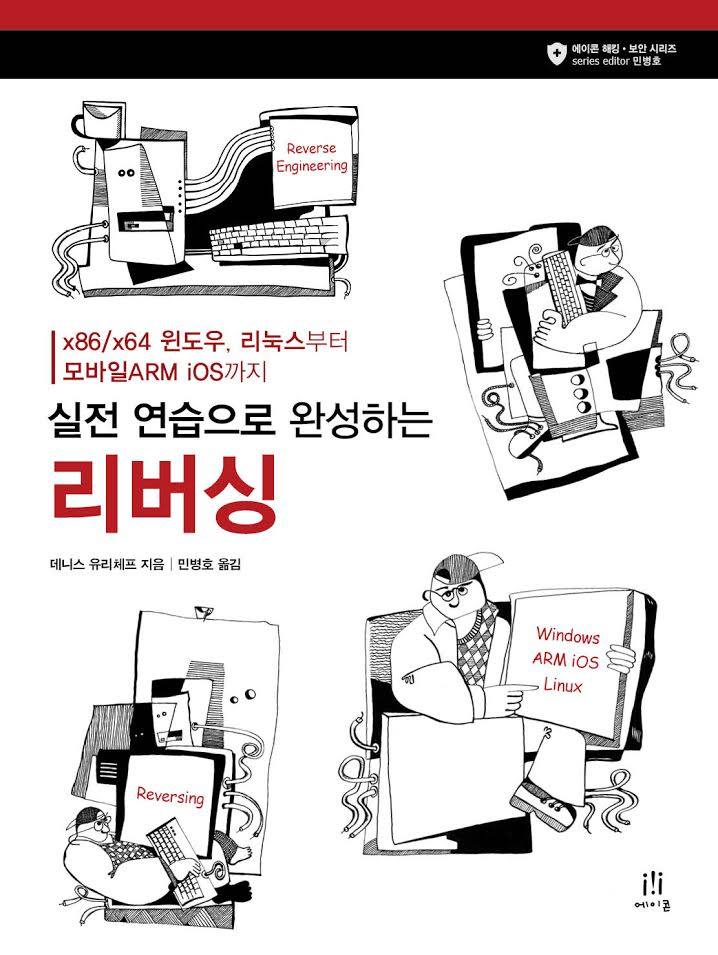
\includegraphics[scale=0.3]{acorn_cover.jpg}
\end{figure}
\fi

The translator is Byungho Min (\href{http://go.yurichev.com/17344}{twitter/tais9}).
The cover art was done by my artistic friend, Andy Nechaevsky:
\href{http://go.yurichev.com/17023}{facebook/andydinka}.
They also hold the copyright to the Korean translation.

So, if you want to have a \IT{real} book on your shelf in Korean and 
want to support my work, it is now available for purchase.

